\documentclass[a4paper, 11pt]{article}

\usepackage[french]{babel}
\usepackage[utf8]{inputenc}
\usepackage[T1]{fontenc}
\usepackage{placeins}
\usepackage{csquotes}
\usepackage{hyperref}
\usepackage{graphicx}

\graphicspath{{img/}}

\author{Florian Thuin \and Cyril de Vogelaere}
\date{\today}
\title{Assignment 2 : Deeper understanding of j-- compiler}

\begin{document}
    \maketitle
    \tableofcontents
    \section{Lexical analysis}
    \section{Parsing}
    \section{DFA}
    	Yes, it is possible to accept an infinite language, for example
    	((1)* 0) accept an infinite sequence of bit but can be 
    	represented by the following DFA :
    	
    	\begin{figure}[!h]
    		\center
    		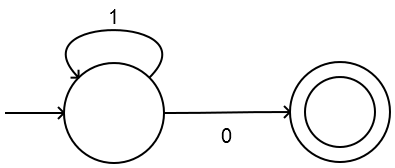
\includegraphics[scale=0.5]{DFAQ3.png}
    	\end{figure}
    	
    \section{Language}
\end{document}
